\documentclass[a4paper, 12pt]{article}
\usepackage[english]{babel}
\usepackage[pdftex]{graphicx}
\usepackage[latin1]{inputenc}
\usepackage[T1]{fontenc}
\usepackage{hyperref}
\usepackage{listings}


\setlength{\parindent}{0.0in}
\setlength{\parskip}{0.1in}

\setcounter{secnumdepth}{5}
\setcounter{tocdepth}{5}


\makeatletter
\renewcommand{\paragraph}{\@startsection{paragraph}{4}{0ex}%
   {-3.25ex plus -1ex minus -0.2ex}%
   {1.5ex plus 0.2ex}%
   {\normalfont\normalsize\bfseries}}

\renewcommand{\subparagraph}{\@startsection{subparagraph}{5}{0ex}%
   {-3.25ex plus -1ex minus -0.2ex}%
   {1.5ex plus 0.2ex}%
   {\normalfont\normalsize\bfseries}}
      \def\clap#1{\hbox to 0pt{\hss #1\hss}}%


\def\ligne#1{%
  \hbox to \hsize{%
    \vbox{\centering #1}}}%

\def\bovenaan#1#2#3{%
  \hbox to \hsize{%
    \rlap{\vtop{\raggedright #1}}%
    \hss
    \clap{\vtop{\centering #2}}%
    \hss
    \llap{\vtop{\raggedleft #3}}}}%

\def\onderaan#1#2#3{%
  \hbox to \hsize{%
    \rlap{\vbox{\raggedright #1}}%
    \hss
    \clap{\vbox{\centering #2}}%
    \hss
    \llap{\vbox{\raggedleft #3}}}}%

\def\maakvoorblad{%
  \thispagestyle{empty}\vbox to \vsize{%
    
    \bovenaan{}{}{}
    
    \vfill
    
    \hrule height 2pt
    \par
	  \begin{center}
	     \Huge \strut \@titel \par
	  \end{center}
    \hrule height 2pt
		\par

    \vspace{13mm}
    
    \ligne{\Large \@auteur}
    \vspace{5mm}
    \ligne{\@opleiding}
    
    \vspace{1cm}
    \vfill
    \vfill
    
    \onderaan{\@promotor}{}{\@academiejaar}
    }%
  \cleardoublepage
  }

\def\titel#1{\def\@titel{#1}}	
\def\auteur#1{\def\@auteur{#1}}
\def\opleiding#1{\def\@opleiding{#1}}
\def\academiejaar#1{\def\@academiejaar{Academiejaar: #1}}
\def\promotor#1{\def\@promotor{#1}}

\makeatother

%Default waarden
\auteur{Auteur}
\opleiding{Opleiding}
\titel{Titel}
\academiejaar{Academiejaar}
\promotor{Promotor}


\begin{document}
\auteur{Kwinten Missiaen, Steven Thuriot, Koen van den Dries, Bart Vangeneugden}
\opleiding{Methodologie�n voor Ontwerp van Programmatuur}
\titel{Taskmanager: Iteratie 1}
\academiejaar{2009 - 2010}
\promotor{Tom Holvoet\\Mario Cruz Torres}

\maakvoorblad

\newpage
\thispagestyle{empty}
\mbox{}

\newpage
\maakvoorblad

\newpage

\tableofcontents

\newpage
\section{Introduction}
		This document serves as a documentation instrument for the first Iteration of the MOP Team Assignment.\\
		In the following chapters, the reader will get a general overview of the outer- and inner workings of the application, accompanied by several diagrams. At first, we will discuss the view layer. The user will be explained how the user interacts with the system. Delving deeper, we lay out how packages were used to ensure safe, decoupled and thought-through class-to-class communication.
		Once this is covered, we explain in detail just which classes have which responsibility, and why. Also our testing approach is explained in short.\\
		We conclude with our team organization, planning and a short self-evaluation.
	\section{System Operations}
		\subsection{Task Management}
			The system revolves around Tasks. There are many different entities to keep in mind such as Users, Resources or Projects.
			But all of these things somehow have to do with Tasks itself.
			\subsubsection{Creation of tasks}
				When creating a Task, the User asked to give details about the task at hand. The user is expected to enter a short description, the start time of the task, the deadline and the average duration of the task.
				Also, the user is presented with a list of resources and other tasks already in the system. The user then selects a few dependencies for the task he's creating and resources he wishes to allocate.

				When creating a task, the user has to make sure he does not violate the business rule when creating this Task. This means the user enters a duration, start date and end date. The start date must come before the end date and the difference between end- and start date has to be larger or equal then the duration. Also the systems tests if the entered description is an empty string. If this happens, an error is shown.\\
				\begin{figure}[h!]
					\begin{center}
						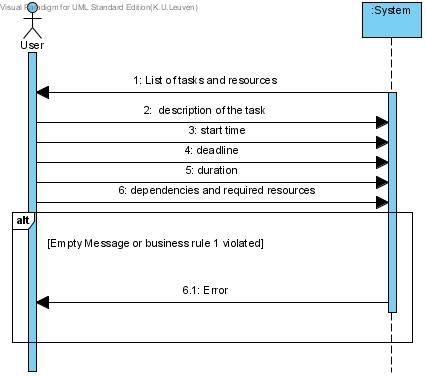
\includegraphics[scale=0.5]{images/ssd_create_task.jpg}
					\end{center}
					\caption{System Sequence Diagram describing the creation of a task}
				\end{figure}
			\subsubsection{Removing Tasks}
			When a task is to be removed. It first has to check how that will affect other entities in the system. Is a Task still required by other Tasks in a dependency?
			If this is the case. The user will receive an error message and is asked how he wants to proceed: Cancel the operation or delete all the dependent tasks.
			\begin{figure}[h!]
				\begin{center}
					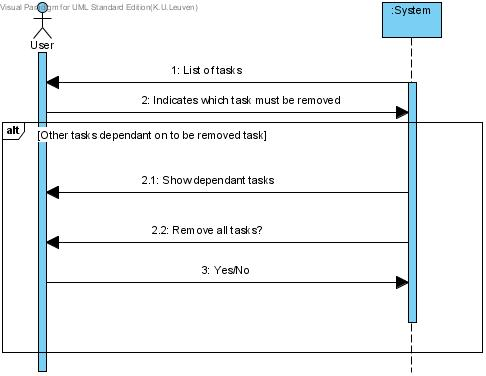
\includegraphics[scale=0.5]{images/ssd_remove_task.jpg}
				\end{center}
				\caption{System Sequence Diagram describing the removal of a task}
			\end{figure}
			\subsubsection{Modifying Tasks}
			When modifying tasks, the system has to make sure the user follows all the rules described above. This is because the user has the option to change all of the schedule variables, dependencies and required resources.

			This means that the Business Rule has to be tested, as well as the Empty Description rule. Checking is also done on the task dependencies. For instance, it should not be possible to create a task A, dependent on task B. And modify task B to be dependent on task A. This would create a dependency loop.\\
			\begin{figure}[h!]
				\begin{center}
					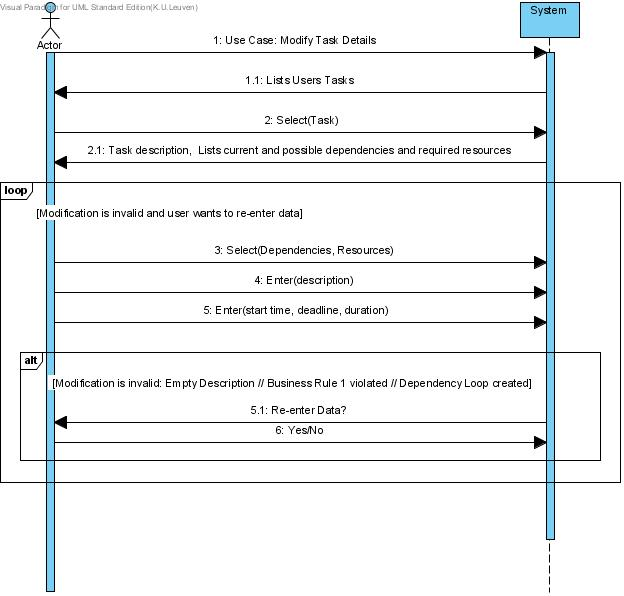
\includegraphics[scale=0.5]{images/ssd_modify_task.jpg}
				\end{center}
				\caption{System Sequence Diagram describing the editing of a task}
			\end{figure}
			 \subsubsection{Updating a Task status}
			Updating a status of a task is integrated in modifying a task, but requires special attention as many different rules apply when adjusting the status of a Task.

			Updating the status can directly reflect the status of dependent tasks. When a task is marked as successful, the user may select if he wants the dependent tasks to be marked as Successful as well.
			The reason for this is because a Task can only 'be' successful if the task, and all of it's dependencies have been executed correctly.
			\begin{figure}[h!]
				\begin{center}
					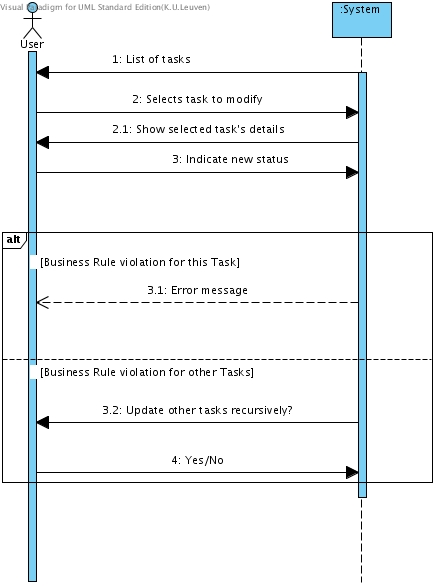
\includegraphics[scale=0.5]{images/ssd_update_task.jpg}
				\end{center}
				\caption{System Sequence Diagram describing the updating of the status of a Task}
			\end{figure}
		\subsection{Resource Management}
			\subsubsection{Creating Resources}
			A user can create a resource. When this resource is created, it is added to the system and stored there for later use.
			The system will only check for a valid description. This means the description can not be empty.

			Once created, the resource is available for binding to Tasks, or Reservations.
			\subsubsection{Remove Resource}
			A Resource can be removed. However, the system will first check it's dependency's with Task objects and/or Reservations.
			If the Resource is required by any of these, the system can not remove the Resource.
		\subsection{Reservations}
			\subsubsection{Create Reservations}
			Once a Resource is created, the User has the option to make a Reservation for that Resource.
			When creating a Reservation, the user is asked for the period of time he wants to make the Reservation after being shown a list of current Reservations for the Resource.

			After the user enters this data, the system controls the entered data to see if it does not conflict with previous Reservations.
		\subsection{Project Management}
			\subsubsection{Create Project}
			A project can be created. A project can contain many Tasks, but does not have to. Our assumption is that at least one User is allocated to a Project, but several Users can subscribe.
			The system asks the user for a short description of that Project. If this description was not empty, the system creates the Project.
			\subsubsection{Remove Project}
			A project can be removed without too many details. If the user wants to remove a project, all of the tasks connected to that project are removed. The user simply selects a Projects and all of the underlying tasks/dependent tasks are removed with it.
	\section{Subsystem Descriptions}
		\subsection{User}
		The system evolves around the User. The user can be considered the Information Expert.
		When starting with a User object, almost the entire Object hierarchy can be described.

		We looked and discussed the model and responsibility of the User-class from many different angles. We came to the conclusion that the User of the System represents the User in the system. Therefore all of the Tasks, Reservations he creates in a way 'belong' to him.

		However not described, we assumed the system could become a multi-user system in the next iteration(s). We therefore based our design on this.
		\subsection{Task manipulation}
			%Design uitleggen. Ook de GRASP patterns erbij zetten
			\subsubsection{Design}
			Tasks are collected in the User. They contain a list of Resources the User might require to execute the Task.
			A Task has attributes which define it's own description, a Start and End time as well as a Duration.
			Also, a Task has a list of Tasks on which the Task may depend. This means the status of the Task at hand is dependent on the Status of it's dependent Tasks.\\
			Keeping Low Coupling and High Cohesion in mind, Task has the following responsibilities:
			\begin{itemize}
				\item{Collecting Resources}
				\item{Keep a recursive dependency list}
				\item{Check for the business rule recursively}
				\item{Check for the Task status recursively}
			\end{itemize}
			A Task is not however an Information Expert or Creator of Resources. As described in the next chapter, a Resource has it's own management.
			We do feel it is necessary for the Task to know about it's Resources.\\
			A Task is Information Expert about Task itself. It makes sure the dependent Tasks as (recursively) correct according to the Business Rule. This means a Task can only be 'successful' when it's dependencies are 'successful'. Also end times of Tasks have to match earlies end times of dependent Tasks.			
			%Functionaliteiten beschrijven
			\subsubsection{Functionality}
			
			%Klasses met hun verantwoordelijkheden beschrijven
			\subsubsection{Class Descriptions}
			
		\subsection{Resource manipulation}
			%Design uitleggen. Ook de GRASP patterns erbij zetten
			\subsubsection{Design}
			Resources can be accessed via Tasks. This is because a Task can define which resources are required for that Task.
			However when a Resource is just created, or when a Task to which a Resource was allocated gets removed, the Resource has no more place in an Object Oriented structure. The object would not exists.
			Therefore we decided to keep a reference of each Resource in a class with a static instance.

			A Resource itself is in Information Expert as well as a Creator for Reservations. We decided to put the responsibility of creating and storing Reservations in Resource because a Resource needs this information to check it's own availability as seen in the following diagram Create Reservation.
			\begin{figure}[h!]
				\begin{center}
					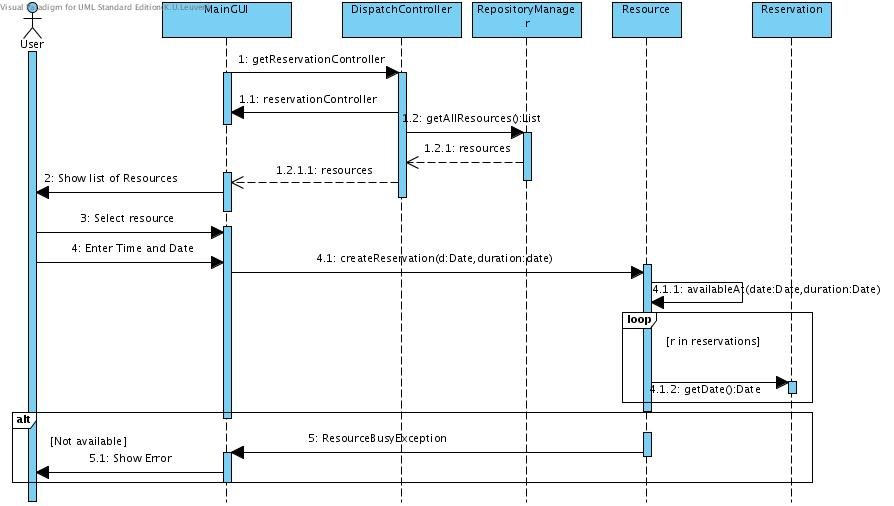
\includegraphics[scale=0.5]{images/create_reservation.jpg}
				\end{center}
				\caption{Create Reservation Sequence Diagram}
			\end{figure}

			As shown in the diagram 'Create Reservation Sequence Diagram', all the Resources are retrieved from the Singleton ResourceManager. Once selected, a Resource can check it's own availability. When available the Resource itself creates the Reservation.

			The OO-structure is shown in the class diagram: Resource Class Diagram which contains all the necessary classes for the Resource subsystem.
			
			\begin{figure}[h!]
				\begin{center}
					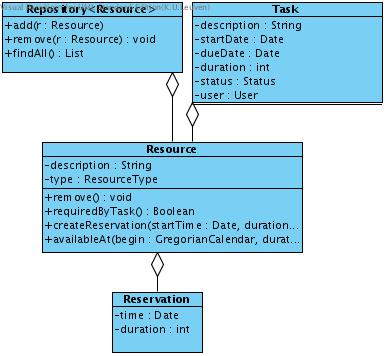
\includegraphics[scale=0.5]{images/resource_class_diagram.jpg}
				\end{center}
				\caption{Resource Class Diagram}
			\end{figure}
		\subsection{Project manipulation}
			When we assumed the project could become a multi-user application. We thought of Projects as a link between multiple Users and Tasks. Therefore, a Project can contain multiple Tasks, and multiple Users can be assigned to it.
			\begin{figure}[h!]
				\begin{center}
					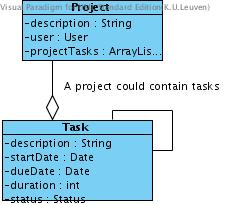
\includegraphics[scale=0.5]{images/project_class_diagram.jpg}
				\end{center}
				\caption{Project Class Diagram}
			\end{figure}
			When the application user creates a Project, he becomes a owner of that Project, this is how the User acts as a container of the Project Object. Tasks can be added to the Project however the User wishes to do this. However, it's not the User object that calls the Project constructor. It is our opinion that it is not the User's responsibility to create this object, rather then it's the Project's responsibility to aggregate the User.
			\begin{figure}[h!]
				\begin{center}
					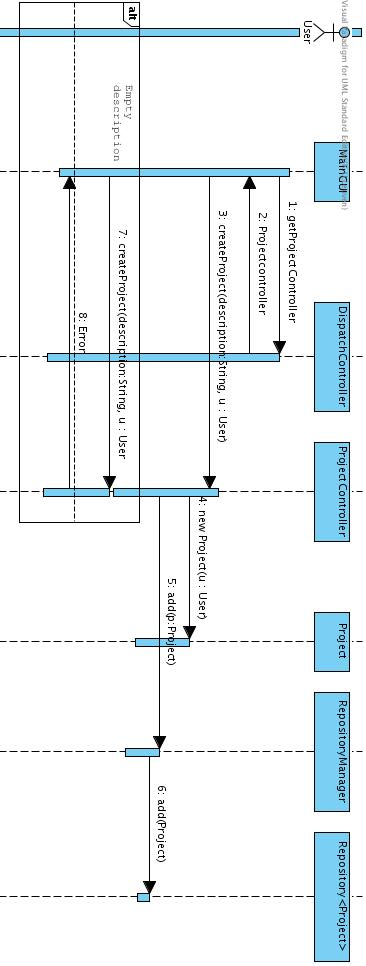
\includegraphics[scale=0.5]{images/create_project.jpg}
				\end{center}
				\caption{Create Project Sequence Diagram}
			\end{figure}
			Therefore, it's the Project's constructor that gets an argument User. This User object is then asked to add Project to it's list of Projects.
			\begin{figure}[h!]
				\begin{center}
					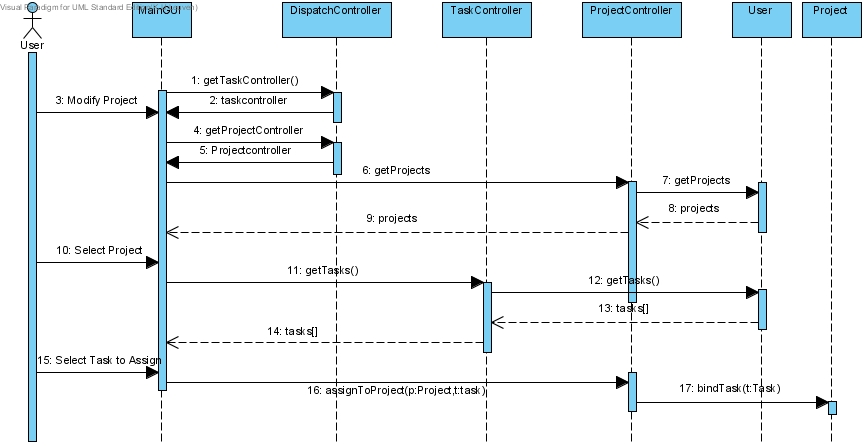
\includegraphics[scale=0.5]{images/assign_task_to_project.jpg}
				\end{center}
				\caption{Assign Task to Project Sequence Diagram}
			\end{figure}
			It is also the Project's responsibility to bind a Task to the Project. We feel that this direction should be maintained because a Project 'contains' or 'aggregates' a Task. This binding is done in the Project's constructor.			
			
	%Welke delen moeten allemaal gewijzigd worden moest er iets veranderen aan de hierarchie?
	\section{Class Descriptions}
		
	\section{Testing}
		\subsection{Technology}
		We decided to use JUnit4 for testing.
		JUnit4 has a few advantages compared to JUnit3. It uses annotations to define a Test. This gives the developer an easy solution to testing for Exceptions.
		\subsection{Testing Approach}
		We decided to go for a defensive and multi-level testing approach.
		By multi-level we mean that we test both methods in Model classes (such as User, Task, Resource etc.) as well as testing the Controllers that call these methods (TaskController, ResourceController etc). 
		This way we get a good view on where errors are: model, controller or view.\\
		We also tested most methods for both cases. This means that we test both failure and succession of a method. Testing only for success does not guarantee a correct Exception is thrown, or success in all cases.
	\section{Project Management}
		\subsection{Planning}
		The planning of our Team Assignment had the following planning:\\
		\begin{tabular}{p{200 pt}|c|c}
		Activity & From & To\\
		\hline
		First meeting \& Discussion of our views on the project & 9/10/2009 & 9/10/2009\\ \hline
		Creation of a draft class diagram \& working out System Sequence Diagrams & 9/10/2009 & 12/10/2009\\ \hline
		First meeting with our advisor. & 12/10/2009 & 12/10/2009\\ \hline
		Individual rework of Class Diagram & 12/10/2009 & 14/10/2009\\ \hline
		Comparing results and creation of definitive Class Diagram & 14/10/2009 & 14/10/2009\\ \hline
		Creation of Sequence Diagrams & 14/10/2009 & 16/10/2009\\ \hline
		Development of Model classes and Controller classes. Building of GUI structure & 16/10/2009 & 19/10/2009\\ \hline
		Code review by team and rewriting certain functionality's & 19/10/2009 & 26/10/2009\\ \hline
		Start writing report \& finishing UML diagrams & 24/10/2009 & 27/10/2009\\ \hline
		\end{tabular}
		\subsection{Teamwork}
		We focused on a close teamwork. We started the project with a team discussion on how everyone saw the project and interpreted the assignment. This gave the team a general perspective and good grasp on how we wanted to implement it.\\
		We have 3 weekly physical meetings, where 1 would be with our team advisor. In these meetings, we discussed what everyone had done in the past days. Whenever somebody was unclear, or the group had doubts about which method or pattern would be the best to use, time was never an issue to come to a general solution that seemed best to everyone.\\
		We also used several team collaboration tools provided by Google such as Google Code and Google Groups. This gave advantages such as a mailing list, subversion with the option to review code at each revision, issue lists and hosted files.\\
		We tried to keep all the information as centralized as possible by using a separate Subversion repository for the Visual Paradigm file. This way every team member always had the most up to date diagrams available.\\
		Development of the project was divided in 4 groups of functionality: Controllers, Models, View and Testing. Each member of the team was assigned one of these tasks. Steven Thuriot took on Controllers and the parsing of XML, Kwinten Missiaen Models, Koen Van Den Dries the View and Bart Vangeneugden Testing. The report was structured and drafted by Bart Vangeneugden however every team member wrote about the part of development he was responsible for.
	\section{Self-Evaluation}
	It is our opinion that we had a great team effort. However, we can improve. In this iteration we were too eager to get a first version of Class- and other diagrams ready. It would have been a better choice to make a good class-per-class analysis before drawing.\\
	To conclude we had no real problems regarding teamwork. Also we learned a lot about project organization.
\end{document}